\newpage
\chapter{State of the art review}
\label{sec:related_work}

Counting the number of an object of interest in an image can be approached from two different perspectives, either training an object detector, or training an object counter\cite{segui2015learning}. In the first case, we must provide the system with a large set of object examples, properly and almost in all cases manually labeled and localized in a way that represent most of the possible views and appearances of the object. The result is a sophisticated object classifier based on manually-crafted features\cite{viola2004robust, viola2005detecting}. In the latter case, we only need to provide the number of object instances for each image sample and the result is typically a regressor\cite{lempitsky2010learning}.  

Recently, with the success of CNNs in different vision tasks, object detection systems based on deep CNN have made groundbreaking advances on several object detection problems\cite{zhang2015improving, erhan2014scalable, girshick2014rich, he2015spatial, erhan2014scalable} which suggests the use of this technique to learn to count objects. Several advantages can be foreseen from this application, being the most important that of learning image features from samples instead of hand-crafting highly specialized image features that are dependent on the object class\cite{segui2015learning}. Moreover, CNN have shown their capacity of knowledge transfer for a number of tasks or the ability of simultaneously performing different tasks even when trained for only one \cite{zhou2014learning}. 

Following this line of work, \citefullauthor{segui2015learning} in \cite{segui2015learning} proposed a novel approach for counting objects' representations using deep object features. In their work, objects' features are learned by a deep counting convolutional neural network and are used to understand the underlying representation. To this end, they define a counting problem for even digits using \textit{MNIST} data and demonstrate that the internal representation of the network is able to classify digits in spite of the fact that no direct supervision was provided for them during training. Moreover, they present preliminary results about a deep network that is able to count the number of pedestrians in a scene\cite{segui2015learning}. Figure~\ref{fig:santimnist} illustrates their proposal at a glance in the case of representing hand-written digits:
\begin{figure}[h!]
	\centering
	{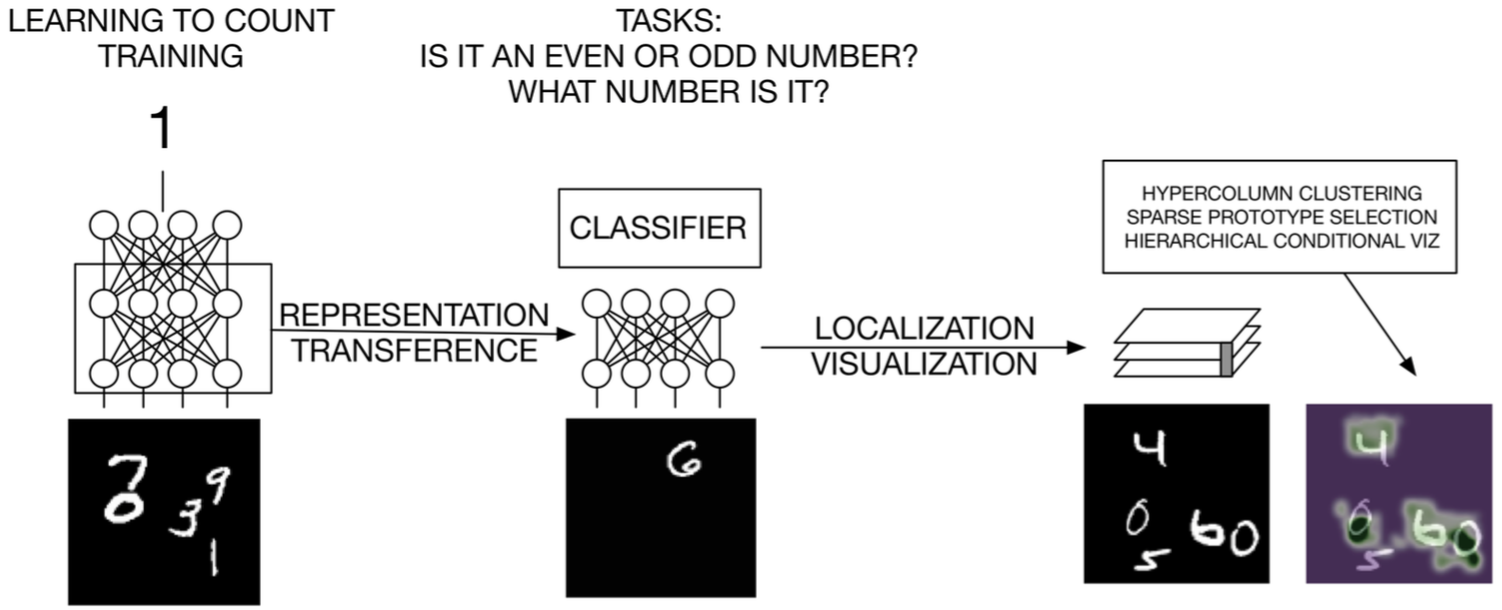
\includegraphics[width=0.6\textwidth]{images/santimnist}}
	\caption{Learning to count hand-written digits problem in which the features of a CNN that has been trained to count digits can be readily used for more specific classification problems and even to localize digits in an image\cite{segui2015learning}.}
	\label{fig:santimnist}
\end{figure}


In \cite{segui2015learning}, the main hypothesis is that the number of occurrence of objects in an image provide strong presentational information due to their possible discriminate appearance for a feature learning process to exploit. In order to verify this hypothesis, for both experiments, they considered networks of two or more convolutional layers (since CNNs instinctively handle feature learning\cite{lecun1989backpropagation}) consisting of convolutional filters, ReLU non-linearities, max-pooling layers and normalization layer,   followed by one or more fully connected layers (regarding the impressive classification performance on different benchmark problems\cite{krizhevsky2012imagenet, Karpathy_2014_CVPR, ciresan2011flexible})\cite{segui2015learning}. 







  


%\cite{paragios2001mrf, cho1999neural, regazzoni1996distributed, davies1995crowd, kong2005counting, marana1998efficacy, viola2004robust}. 

